\documentclass{standalone}
\usepackage{pgfplots}
\newcommand{\point}[2]{\pgfextractx{\dimen0}{\pgfpointdiff{\pgfpointanchor{origin}{center}}{\pgfpointanchor{#1}{#2}}}\pgfextracty{\dimen2}{\pgfpointdiff{\pgfpointanchor{origin}{center}}{\pgfpointanchor{#1}{#2}}}\typeout{POINT #1.#2: \the\dimen0,\the\dimen2}}
\begin{document}
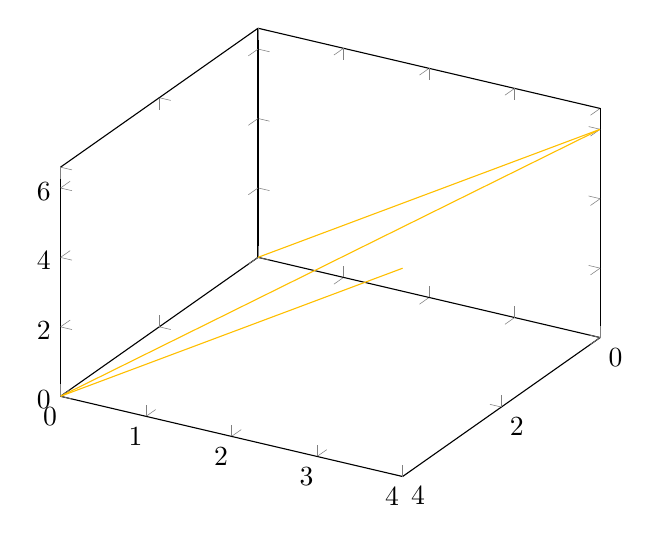
\begin{tikzpicture}
\begin{axis}[view={120}{35},xmin=0,xmax=4,ymin=0,ymax=4,zmin=0,
  xticklabel style={name=xt},yticklabel style={name=yt},zticklabel style={name=zt}]
\addplot3[surf] coordinates {(0,0,0) (0,4,6) (4,0,0) (4,4,6)};
\coordinate (origin) at (axis description cs:0,0);
\coordinate (extent) at (axis description cs:1,1);
\end{axis}
\point{extent}{center}
\point{xt}{center}\point{yt}{center}\point{zt}{center}
\point{current bounding box}{south west}\point{current bounding box}{north east}
\end{tikzpicture}
\foreach \style/\az/\el/\xx/\yy/\zz/\tt in {
 left/335/35/{$x$}/{$y$}/{$xy$}/{Bilinear surface},
 right/55/35/{$x$}/{$y$}/{$T$}/{Temperature field},
 horizontal/45/30/{Stage}/{Queue}/{Load}/{Workflow load}}{
\typeout{CASE parent-\style}
\begin{tikzpicture}
\begin{axis}[name=parent,width=8cm,height=6cm,view={\az}{\el},
 xmin=-1,xmax=1,ymin=-1,ymax=1,zmin=-1,zmax=1,
 xlabel=\xx,ylabel=\yy,zlabel=\zz,title=\tt]
\addplot3[surf,samples=3,domain=-1:1] {x*y};
\coordinate (origin) at (axis description cs:0,0);
\end{axis}
\point{parent}{left of north west}
\point{parent}{right of north east}
\point{parent}{below south west}
\end{tikzpicture}}
\end{document}
